\subsection{Overview}\label{chapter_OVERVIEW}
This chapter leads once through the control loop, that is pictured below.
\begin{figure}[H]
	\centering
		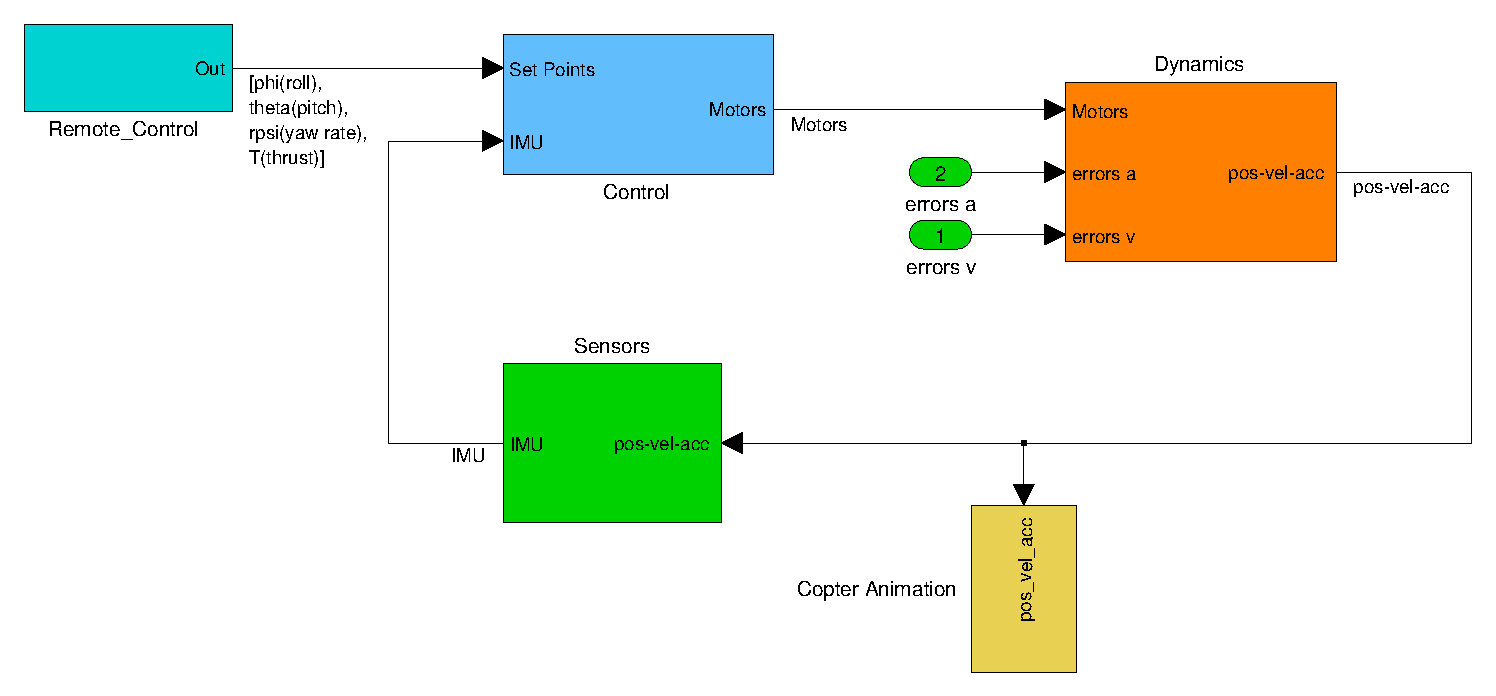
\includegraphics[width=1.0\textwidth]{03_Grafiken/MATLAB_Overview.pdf}
	\caption{Overview Closed Loop}
	\label{fig:MATLAB Overview}
\end{figure}
The cyan-colored block top left, represents the remote control. This block 'generates' the set points. These set points are combined in one vector, consisting of:
\begin{enumerate}
	\item the angle of \textit{phi} (roll)
	\item the angle of \textit{theta} (pitch)
	\item the angular rate of \textit{psi} (yaw rate)
	\item the average motorspeed (thrust)
\end{enumerate}
The next block, colored blue, is the controller block. The state space controller, developed in this project, gets implemented in this block. In there, the set points, given by the first block, get 'converted' into actuating variables. Again, these variables are combined in one vector, consisting of the four pseudo forces.\\
This vector is connected to the input of the next (orange) block, that represents the quadrocopter. Symbolic blocks represent the physical characteristics of the copter. So this block calculates, how the speed of each motor affects the movement of the copter. The result is a big vector called 'pos-vel-acc', which stands for 'positions-velocities-accelerations'. So this vector consists of all states of the quadrocopter, meaning the actual angle of \textit{phi}, \textit{theta}, \textit{psi}; its angular \textit{rate of phi}, \textit{theta}, \textit{psi}; its actual position in \textit{x}, \textit{y}, \textit{z} of the earthframe, and so on. The complete vector is pictured in chapter \ref {chapter_DYNAMICS_BLOCK}.
This vector is the input of the next block of the closed loop - the sensors block, pictured in green - which returns the measured variables, combined in the vector 'IMU' (Inertial Measurement Unit). This vector consists of:
\begin{enumerate}
	\item acceleration in direction of \textit{x} of the bodyframe
	\item acceleration in direction of \textit{y} of the bodyframe
	\item the angular \textit{rate of phi} (roll rate)
	\item the angular \textit{rate of theta} (pitch rate)
	\item the angular \textit{rate of psi} (yaw rate)
\end{enumerate}
Also connected to the vector 'pos-vel-acc' is the yellow block at the bottom of the model. This block includes the animation of the quadrocopter. Though, this is not a real part of the control loop, it is an important assistance for testing the controller, because it allows to fly the quadrocopter virtually.

The next subchapters will walk once through this whole process, described above, starting with the remote control block.